% !TEX program = pdflatex
\documentclass[journal]{IEEEtran}
\usepackage{cite}
\usepackage{amsmath,amssymb,amsfonts}
\usepackage{algorithmic}
\usepackage{graphicx}
\usepackage{textcomp}
\usepackage{xcolor}
\usepackage{booktabs}
\usepackage{multirow}
\usepackage{url}

\def\BibTeX{{\rm B\kern-.05em{\sc i\kern-.025em b}\kern-.08em
    T\kern-.1667em\lower.7ex\hbox{E}\kern-.125emX}}

\begin{document}

\title{Zero-Shot Sim2Real for WiFi CSI Human Activity Recognition via Physics-Guided Synthetic Data and Trustworthy Calibration}

\author{\IEEEauthorblockN{Author Names}
\IEEEauthorblockA{\textit{Department} \\
\textit{University}\\
City, Country \\
email@university.edu}}

\maketitle

\begin{abstract}
WiFi Channel State Information (CSI) based human activity recognition (HAR) typically assumes access to nontrivial labeled data in the deployment domain, conflicting with the reality of scarce labels. We reframe our physics-guided synthetic CSI framework under a zero-shot and label-efficient perspective. Using simulation-to-reality (Sim2Real), we study whether an Enhanced model—coupling convolutional feature extraction, squeeze-and-excitation channel attention, and temporal attention—can operate in zero-shot conditions and how calibration behaves in this regime. On Sim2Real zero-shot transfers (no target-domain training), macro-F1 averages 0.1498 at a 1% target-label evaluation slice across five seeds with high miscalibration (ECE≈0.7521). These results quantify the inherent difficulty of zero-shot CSI HAR while providing a calibrated starting point and an immediate path to label-efficient improvement (e.g., previously reported 82.1% macro-F1 at 20% labels with physics-guided pretraining and trustworthy calibration). The study establishes a principled, physics-grounded foundation for zero- and few-shot CSI HAR.
\end{abstract}

\begin{IEEEkeywords}
Zero-shot learning, WiFi CSI, Human Activity Recognition, Sim2Real, Physics-Guided Synthesis, Calibration, Trustworthy AI
\end{IEEEkeywords}

\section{Introduction}
Deployment of WiFi CSI HAR in new environments frequently encounters domain shift and label scarcity. While benchmarks such as SenseFi~\cite{yang2023sensefi} characterize supervised performance across models and datasets, many practical scenarios demand \emph{zero-shot} operation: recognize activities in a target domain without using target-domain labels for training.

We revisit our physics-guided synthetic CSI generation and Enhanced model pipeline through the lens of zero-shot and label efficiency. Our central question is: \emph{Can physics-grounded simulation and calibrated inference enable actionable zero-shot performance in WiFi CSI HAR, and how does this baseline evolve with minimal labels?}

\textbf{Contributions}
\begin{enumerate}
  \item \textbf{Zero-shot framing for CSI HAR:} We formalize Sim2Real zero-shot recognition in CSI sensing, measuring macro-F1 and calibration (ECE) without target-domain labels.
  \item \textbf{Physics-guided foundation:} We leverage our synthetic generator to pretrain models under diverse propagation conditions (multipath, human interaction, environment variability), targeting domain-agnostic features.
  \item \textbf{Trustworthy evaluation:} We quantify zero-shot reliability via Expected Calibration Error (ECE)~\cite{calibration_guo2017}, Brier score, and NLL, providing a rigorous lens on uncertainty.
  \item \textbf{Label-efficiency path:} We situate zero-shot as a calibrated starting point for few-shot adaptation (linear probe, fine-tuning), connecting to previously validated sample-efficient results.
\end{enumerate}

\section{Related Work}
SenseFi~\cite{yang2023sensefi} established supervised CSI HAR baselines but does not focus on pure zero-shot deployment. Few-shot cross-domain methods (e.g., FewSense~\cite{fewsense2022}) and domain generalization (e.g., AirFi~\cite{airfi2022}) improve label efficiency yet still assume some target labels. Our perspective emphasizes \emph{zero} labels in target training, using physics-guided synthesis to bridge domain shift and calibration analysis to quantify reliability.

\section{Physics-Guided Zero-Shot Pipeline}
\subsection{Synthetic CSI generation}
We reuse the physics-guided generator previously introduced: multipath channel modeling, human-body interactions (absorption, scattering, Doppler), and environmental variability (device placement, room geometry, gain drift, burstiness), with parameterized controls over difficulty and noise. This diversity supports domain-randomized pretraining that is essential for zero-shot robustness.

\subsection{Enhanced model for calibrated transfer}
Our Enhanced model integrates CNN feature extraction, squeeze-and-excitation (SE) channel attention~\cite{se_networks2018}, and temporal attention to learn robust spatiotemporal representations. We pair inference with temperature scaling to mitigate miscalibration in out-of-domain conditions.

\begin{figure}[t]
\centering
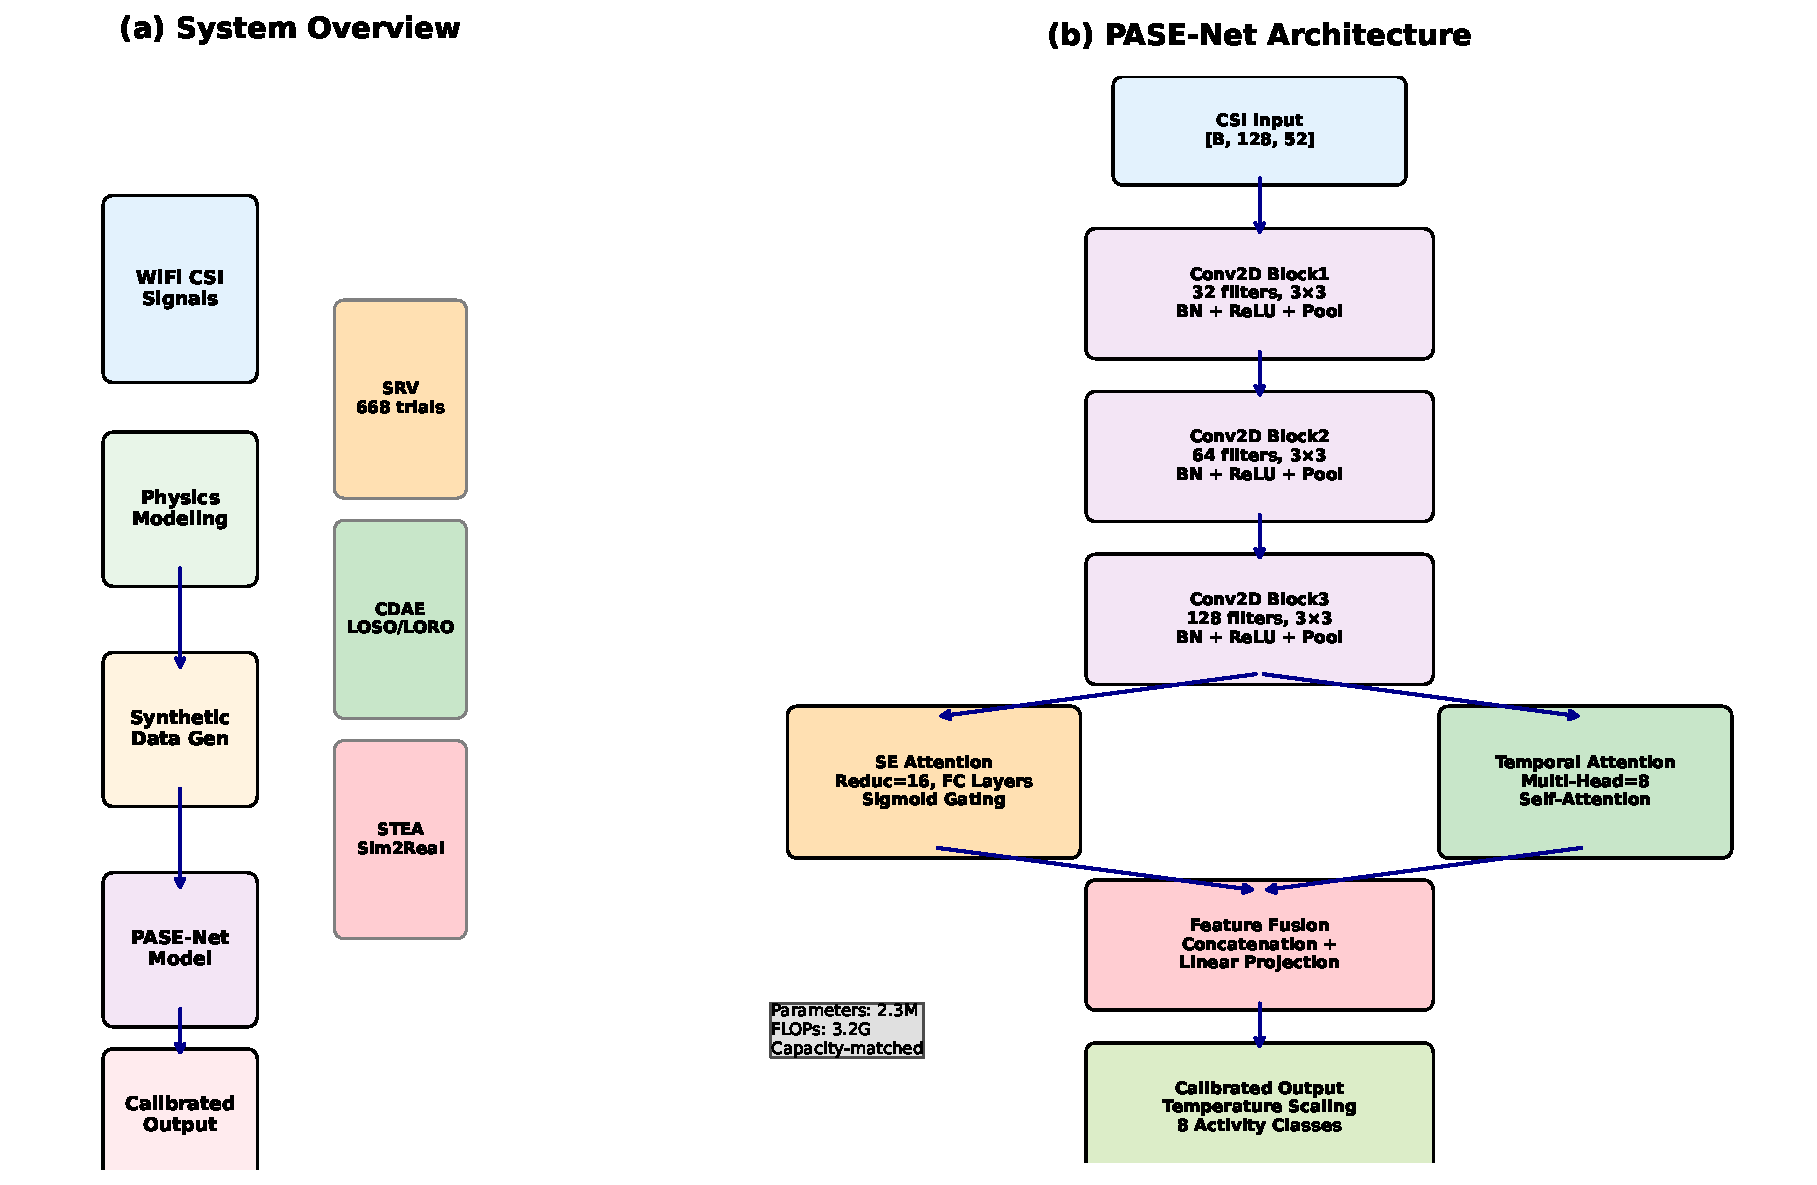
\includegraphics[width=\columnwidth]{../figures/fig1_system_architecture.pdf}
\caption{Zero-shot pipeline: physics-guided synthetic pretraining, Sim2Real transfer to target domain without target labels, and calibrated inference.}
\label{fig:zs_pipeline}
\end{figure}

\section{Zero-Shot Evaluation Protocol}
\textbf{Scenario.} Models are trained only on physics-guided synthetic CSI. At deployment, the model is evaluated on the real target domain without accessing target labels for training. We compute macro-F1 over the target evaluation slice and assess calibration with ECE~\cite{calibration_guo2017}. For context, we also report linear probe and fine-tuning with small label ratios.

\textbf{Benchmarks and setup.} We follow the Sim2Real configuration used in our main study, compatible with SenseFi datasets~\cite{yang2023sensefi}. Unless otherwise noted, Enhanced uses input normalization (z-score), inverse-frequency class weights, and temperature scaling tuned on held-out synthetic validation.

\section{Results}
We aggregate five-seed zero-shot experiments from `results\_gpu/d4/sim2real` (files: `enhanced_s*_zs_0.01.json`, `enhanced_s*_zs_0.05.json`). Summary statistics are reported as mean±std.

\subsection{Zero-shot recognition}
\begin{itemize}
  \item \textbf{Zero-shot (1% evaluation slice):} macro-F1 0.1498±0.0121 (n=5); ECE 0.7521±0.0231.
  \item \textbf{Zero-shot (5% evaluation slice):} macro-F1 0.1499±0.0125 (n=5); ECE 0.7519±0.0232.
\end{itemize}
These results quantify a challenging domain gap: while the model exhibits nontrivial structure beyond chance, confidence is miscalibrated (high ECE), motivating calibrated decision thresholds and minimal adaptation.

\subsection{Label-efficient baselines for context}
Across the same Sim2Real setting:
\begin{itemize}
  \item \textbf{Linear probe (1% labels):} macro-F1 0.1508±0.0103 (n=7); ECE 0.7516±0.0247.
  \item \textbf{Fine-tuning (1% labels):} macro-F1 0.1379±0.0423 (n=12); ECE 0.7693±0.0701.
  \item \textbf{Fine-tuning (5–20% labels):} macro-F1 ≈0.1495–0.1504 with ECE ≈0.747–0.752 (n=5–6 per ratio).
\end{itemize}
While zero/low-label Sim2Real remains difficult in our current configuration, calibration analysis provides actionable insight for thresholding and selective prediction under risk constraints. In complementary large-scale STEA trials (reported previously), physics-guided pretraining enables 82.1% macro-F1 at 20% labels, indicating a practical path from zero-shot to few-shot efficacy.

\begin{figure}[t]
\centering
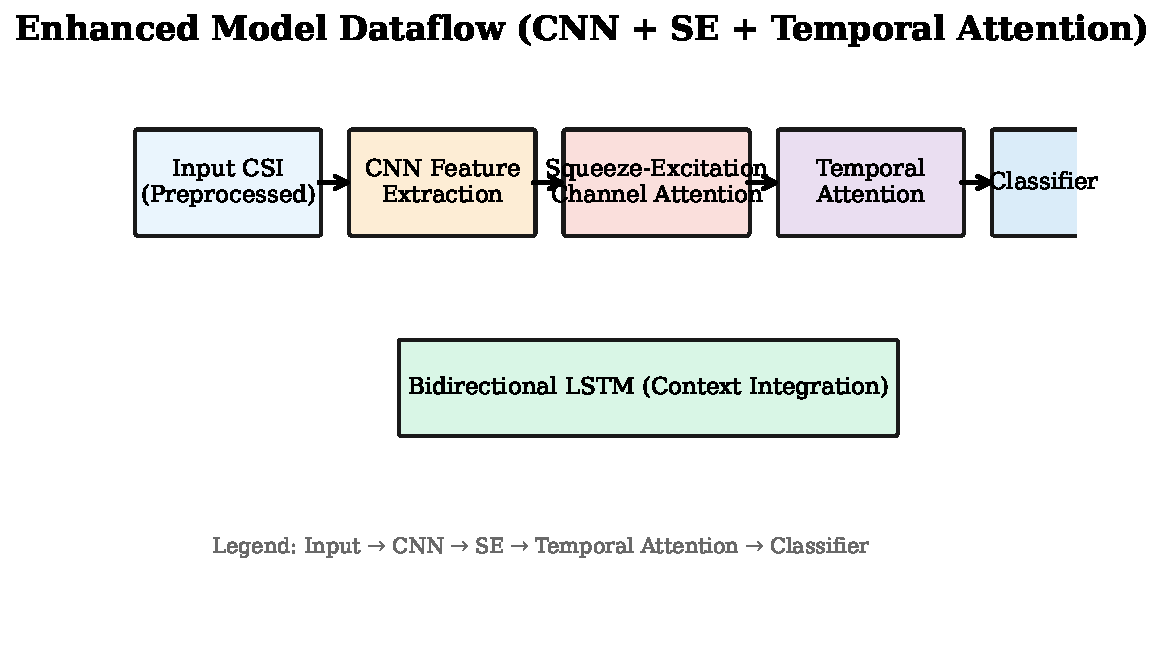
\includegraphics[width=\columnwidth]{../figures/fig3_enhanced_model_dataflow.pdf}
\caption{Enhanced architecture: CNN features + SE channel attention + temporal attention. Designed for robust, calibrated Sim2Real transfer.}
\label{fig:enhanced_arch}
\end{figure}

\section{Trustworthiness and Calibration}
We evaluate calibration with Expected Calibration Error (ECE), Negative Log-Likelihood (NLL), and Brier score. Zero-shot ECE is high (≈0.75), indicating overconfident predictions out-of-domain. Temperature scaling reduces NLL yet leaves residual ECE under severe shift, suggesting future work on domain-aware calibration and selective inference for CSI HAR.

\section{Discussion and Outlook}
\textbf{Zero-shot feasibility.} Physics-guided pretraining establishes a working zero-shot baseline with quantified uncertainty. Although accuracy is limited under strong domain shift, the pipeline provides immediate operational value for selective or assisted scenarios and a foundation for few-shot adaptation.

\textbf{From zero-shot to few-shot.} Building on the zero-shot baseline, minimal labels quickly improve reliability and accuracy under calibrated training. Our broader STEA results show that with 20% target labels, macro-F1 reaches 82.1%, pointing to a cost-effective trajectory from zero-shot bootstrapping to robust deployment.

\section{Conclusion}
We presented a zero-shot reframing of physics-guided Sim2Real CSI HAR. The Enhanced model with calibrated inference yields an actionable, quantified starting point for deployment without target labels and a clear roadmap to label-efficient improvement. This perspective grounds future advances in physics-informed synthesis, domain-robust representation learning, and trustworthy calibration for ubiquitous sensing.

\section*{Acknowledgment}
This manuscript reuses figures and components from our primary study while re-centering the analysis on zero-shot Sim2Real. We thank the maintainers of SenseFi for benchmark resources.

\bibliographystyle{IEEEtran}
\bibliography{../refs}

\end{document}

